% -*- compile-command: "cd .. && make" -*-
\documentclass[document.tex]{subfiles}
\begin{document}

\chapter{Case~Study: Fourth~Year~Project~System}
\label {ch:case-study-1}

The fourth-year project management system is used by the department of Systems and Computer Engineering at Carleton University to manage the completion of fourth-year projects by students in software- and systems-related programs. The system provides students with information on candidate projects, expectations, deadlines and deliverables, and also manages the submission of some project deliverables.

The system fulfills its functional requirements, but requires significant effort on the part of students to navigate, as all actions, information and deadlines are available at all times. It offers a good example of a system where the user experience could be improved by structuring the system into workflows. Additionally, the system involves deadlines and collaborative activities between multiple actors, which makes it a good test of the capabilities of the Stonepath workflow framework.

\sectionnote {BM}
\section {Requirements}
\label {sec:4ys-requirements}

The fourth-year project management system is used by three types of actors:
\begin{itemize}
\item the \keyword{Project Coordinator}, who is an instructor responsible for overall administration of the fourth-year projects and events;
\item \keyword{Project Supervisors}, which are instructors who suggest candidate projects and supervise the completion of individual projects; and
\item \keyword{Project Group Members}, which are students who must be members of exactly one project group.
\end{itemize}
Additionally, the Project Supervisors supervising a project and Project Group Members who are members of it are also referred to as \keyword{Project Participants}.

These three actors use the system for tasks that can be split into four main concerns, specifically
\begin{itemize}
\item \keyword{setup}, which involves configuring the system for a new slate of projects and groups;
\item \keyword{account management}, which involves creating accounts for Project Supervisors and Project Group Members, as well as authentication with the system;
\item \keyword{project selection}, which entails Project Supervisors creating candidate projects and managing group membership, as well as Project Group Members browsing available projects, consulting with Project Supervisors to find a project, and joining a project; and
\item \keyword{project execution}, which involves all of the collaboration between Project Group Members and the Project Supervisor(s) for their project.
\end{itemize}

Individual use cases for these concerns are illustrated in Figures \ref{fig:case-4ys-use-case-setup} through \ref{fig:case-4ys-use-case-oral-reports}. Note that the project execution concern has been split into its own use case diagram (Figure \ref{fig:case-4ys-use-case-oral-reports}) as its requirements are somewhat more complex than the other phases of the project lifecycle.
Detailed use case descriptions are provided in Appendix \ref{ch:detailed-use-cases-1}.

\begin{figure}[!ht]
\centering 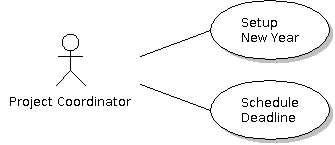
\includegraphics[width=3in]{./img/case-study-fourth-year-system/setup}
\caption{Use case diagram for the setup functionality of the fourth-year project management system.}
\label{fig:case-4ys-use-case-setup}
\end{figure}

\begin{figure}[!ht]
\centering 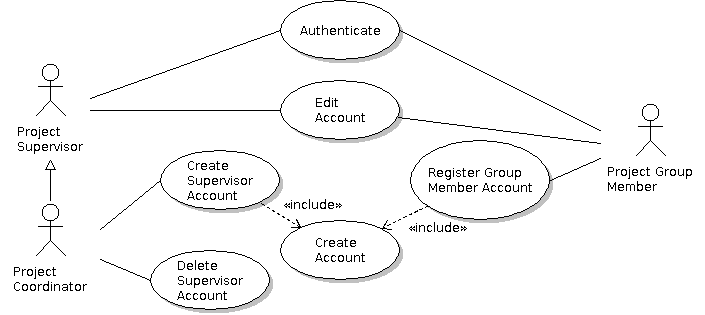
\includegraphics[width=6in]{./img/case-study-fourth-year-system/account-management}
\caption{Use case diagram for the account management functionality of the fourth-year project management system.}
\label{fig:case-4ys-use-case-account-management}
\end{figure}

\begin{figure}[!ht]
\centering 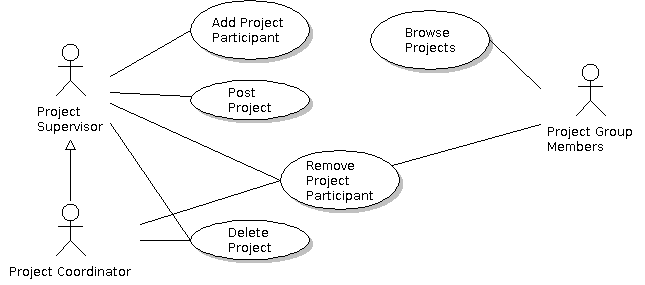
\includegraphics[width=6in]{./img/case-study-fourth-year-system/project-selection}
\caption{Use case diagram for the project selection functionality of the fourth-year project management system.}
\label{fig:case-4ys-use-case-project-selection}
\end{figure}

\begin{figure}[!ht]
\centering 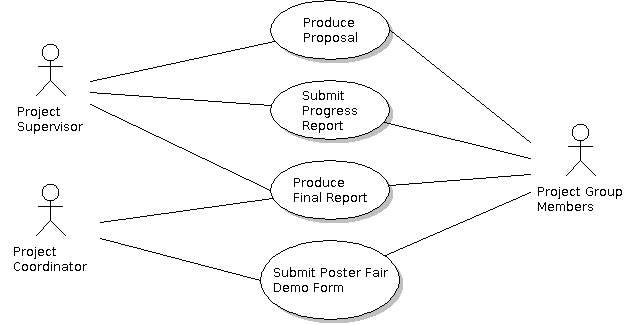
\includegraphics[width=6in]{./img/case-study-fourth-year-system/project-lifecycle}
\caption{Use case diagram for the project execution functionality of the fourth-year project management system. Note that functions related to oral presentations are broken out in Figure \ref{fig:case-4ys-use-case-oral-reports} instead.}
\label{fig:case-4ys-use-case-project-lifecycle}
\end{figure}

\begin{figure}[!ht]
\centering 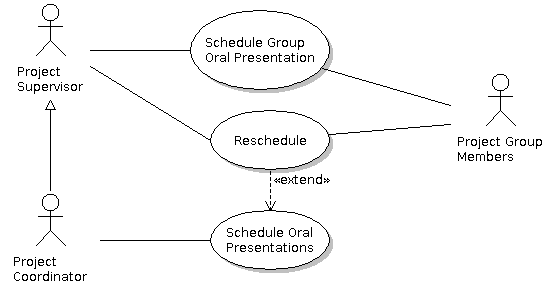
\includegraphics[width=6in]{./img/case-study-fourth-year-system/oral-report-scheduling}
\caption{Use case diagram for the oral presentation functionality of the fourth-year project management system.}
\label{fig:case-4ys-use-case-oral-reports}
\end{figure}


Though all three concerns are important to the system, the most interesting from the point of view of a workflow framework is the project execution phase. This phase accounts for the majority of the lifetime of a fourth-year project, and is also the area in the existing fourth year project management system that could use the most improvement. While account creation and project selection mostly involve basic CRUD (create, read, update, and delete) actions, the execution phase has a well-defined flow:
\begin{enumerate}
\item First, a project proposal must be drafted, submitted, revised, and accepted.
\item After the proposal is accepted, an oral presentation scheduling form must be filled out.
\item Concurrently with scheduling an oral presentation, a progress report must be prepared and submitted.
\item After the progress report is accepted, an oral presentation must be given.
\item After the oral presentation, the group must prepare a presentation for the poster fair. Though this activity has no online deliverables, the group may opt to fill out a poster fair demo request form.
\item While the group is preparing for the poster fair, a final report must also be drafted, submitted, revised, and accepted.
\end{enumerate}
Each step of the fourth-year project process also has associated deadlines.

\FloatBarrier


\sectionnote{BM}
\section{Workflow Design}
\label{sec:4ys-workflow-design}

The six-step project execution phase described in section \ref{sec:4ys-requirements} is the core workflow of a project in the fourth-year project management system. As this high-level workflow is completely linear, it can be trivially transformed into the state chart in Figure \ref{fig:state-machine-project-lifecycle}. In this model, the project is a Stonepath work item, while each step is associated with a set of tasks (ex. producing a proposal or submitting a poster fair demo form), which can be extracted from the use case descriptions in section \ref{sec:4ys-requirements}.

\begin{figure}[!htbp]
\centering \includegraphics[width=3.8in]{./img/case-study-fourth-year-system/project_lifecycle}
\caption{State chart representation of the workflow for an overall project lifecycle from creation to completion.}
\label{fig:state-machine-project-lifecycle}
\end{figure}

In fact, the majority of the tasks described by the use cases involve the Project Group Members submitting an artifact, the Project Supervisor reviewing it, and then either returning it or accepting it. These tasks can be modelled as Stonepath tasks, which may be assigned to Project Group Members and Project Supervisors. This process is captured in Figure \ref{fig:state-machine-document-submission}. This model leverages Stonepath’s state-based model of tasks to handle multiple activities in parallel (ex. filling out the oral report scheduling form, and producing a progress report.)

\begin{figure}[!htbp]
\centering \includegraphics[width=3.0in]{./img/case-study-fourth-year-system/document_submission}
\caption{State chart representation of a general document submission task, such as proposal submission.}
\label{fig:state-machine-document-submission}
\end{figure}

Other tasks to produce deliverables require only some small modifications to the state chart in Figure \ref{fig:state-machine-document-submission}. For instance, the special handling of deadlines for final reports can easily be handled with two extra state transitions, as Figure \ref{fig:state-machine-final-report-submission} demonstrates.

Similarly, the consensus requirement to submit the oral presentation scheduling form only requires a guard clause. On the other hand, it does not make sense to ``return'' a scheduling form if a participant has a conflict; instead, the participant only needs to edit the form and ask the others to approve it again. This workflow is demonstrated in Figure \ref{fig:state-machine-oral-presentation-scheduling}.

\begin{figure}[!htbp]
\centering \includegraphics[width=6.2in]{./img/case-study-fourth-year-system/final_report_submission}
\caption{State chart representation of a the final report submission task. This workflow is an extension of the general document submission workflow in Figure \ref{fig:state-machine-document-submission}, with additional transitions for strict handling of missed deadlines.}
\label{fig:state-machine-final-report-submission}
\end{figure}

\begin{figure}[!htbp]
\centering \includegraphics[width=6.0in]{./img/case-study-fourth-year-system/oral_presentation_scheduling}
\caption{State chart representation of a the oral presentation scheduling task. This workflow is an extension of the general document submission workflow in Figure \ref{fig:state-machine-document-submission}, with additional transitions to handle achieving consensus on available times, editing a submitted form, and closing the form when the deadline expires.}
\label{fig:state-machine-oral-presentation-scheduling}
\end{figure}


\FloatBarrier

\sectionnote{BM}
\section{Design}
\label{sec:4ys-design}

The design of the system was performed in a top-down fashion, starting from the core project workflow depicted in Figure \ref{fig:state-machine-project-lifecycle}. The system must accommodate multiple concurrent tasks for a user: not only can some states involve multiple tasks, but Project Supervisors may be involved with several project simultaneously. The clearest way to present all of the concurrent tasks for a user is in a tabular view, as depicted in the wireframe in Figure \ref{fig:wireframe-tasks-view}. The user can then select a task from their pending tasks, and carry out the actions associated with its present state.

\begin{figure}[!htbp]
\centering 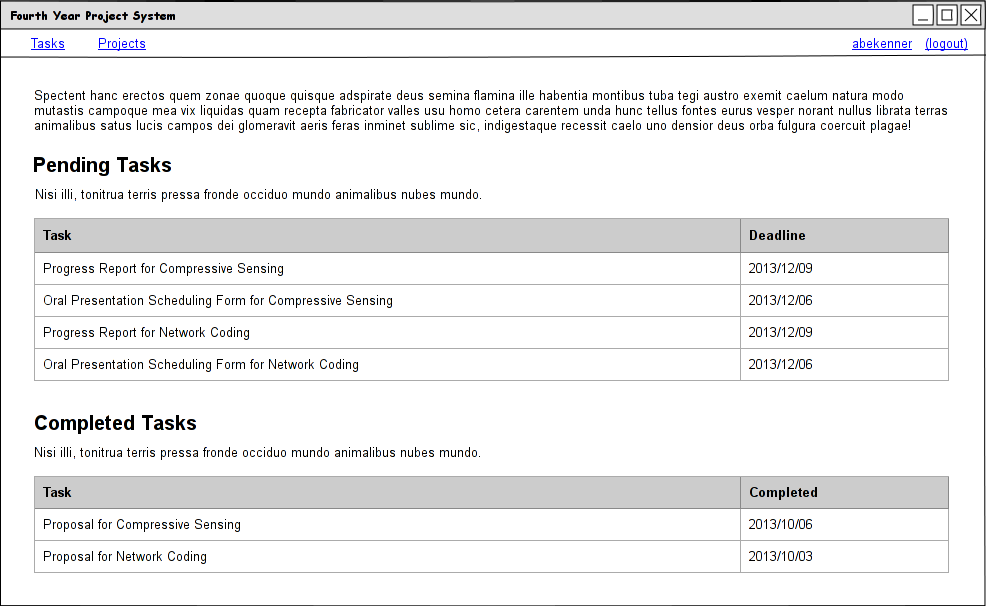
\includegraphics[width=6in]{./img/case-study-fourth-year-system/supervisor-tasks-view_wireframe}
\caption{Wireframe of the tasks view for a Project Supervisor. The tasks view presents the tasks generated by the project state machine in Figure \ref{fig:state-machine-project-lifecycle}. ``Lorem ipsum'' placeholder text has been used in place of introductory and explanatory text.}
\label{fig:wireframe-tasks-view}
\end{figure}

In order to achieve this requirement, the system needs to treat different types of tasks in a project generically - a naive implementation that places each type of task (such as a proposal or progress report) in a discrete ActiveRecord model makes it complex to find all of the outstanding tasks for a user. Stonepath has a SPTask mixin that allows a task to be associated with a workbench (ex. a Project Supervisor) and a workitem (a project). A model extending SPTask might be associated with each task for each workbench / workitem pair, using a polymorphic association. Unfortunately this model is very complex to implement and query, as demonstrated by Figure \ref{fig:sptask-complexity}. Though the relationship between users and tasks is now generic, a polymorphic many-to-many relationship like \verb!Task! is difficult to traverse, as discussed in section \ref{sec:stonepath-prototyping-results}. Additionally, this data model is unnecessarily complex to update in exceptional cases: if a Project Supervisor or Project Group Member needs to be added or removed from the project, then new \verb!Task!s must be added or removed from the database through some means other than the project’s state machine.

\begin{figure}[!htbp]
\centering 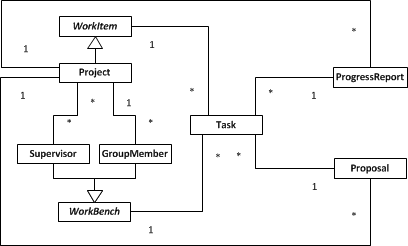
\includegraphics{./img/case-study-fourth-year-system/task-with-sptask-static-structure}
\caption{Logical class diagram of the relationship between concrete tasks of the project workflow (such as proposals and progress reports), projects, supervisors, and group members using Stonepath concepts.}
\label{fig:sptask-complexity}
\end{figure}

Instead of making use of the Stonepath task model, a simpler custom data model was designed instead. As pictured in Figure \ref{fig:custom-task-simplicity}, instances of a new generic \verb!Task! type are associated directly with a project. This is conceptually much simpler, and also allows Project Supervisors and project Group Members to be added and removed from projects without altering the tasks associated with the project.

\begin{figure}[!htbp]
\centering 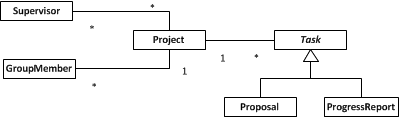
\includegraphics{./img/case-study-fourth-year-system/task-through-project-static-structure}
\caption{Logical class diagram of the relationship between concrete tasks of the project workflow (such as proposals and progress reports), projects, supervisors, and group members using a custom task model.}
\label{fig:custom-task-simplicity}
\end{figure}

With the framework in place to access individual tasks, it was decided that each task in a project would have its own page. In general, task pages are laid out with a detailed task description, followed a short summary of the state of the task, actions that can be performed on the task, and then any other data that is necessary to complete the activity corresponding to the current state of the task. This centralizes information related to a task, and guides the user through the process of completing it. The wireframes in Figures \ref{fig:wireframe-group-member-proposal-view} and \ref{fig:wireframe-supervisor-proposal-view} demonstrate this layout with a proposal task: first, there is a description of the proposal requirements (the task description), followed by a summary of the task state (the file associated with the current submission), actions (``submit'', and ``return'' or ``accept''), and auxiliary data (the submission history.) Note that the actions displayed for the proposal are selected based on the current user's role and the state of the task.

\begin{figure}[!htbp]
\centering 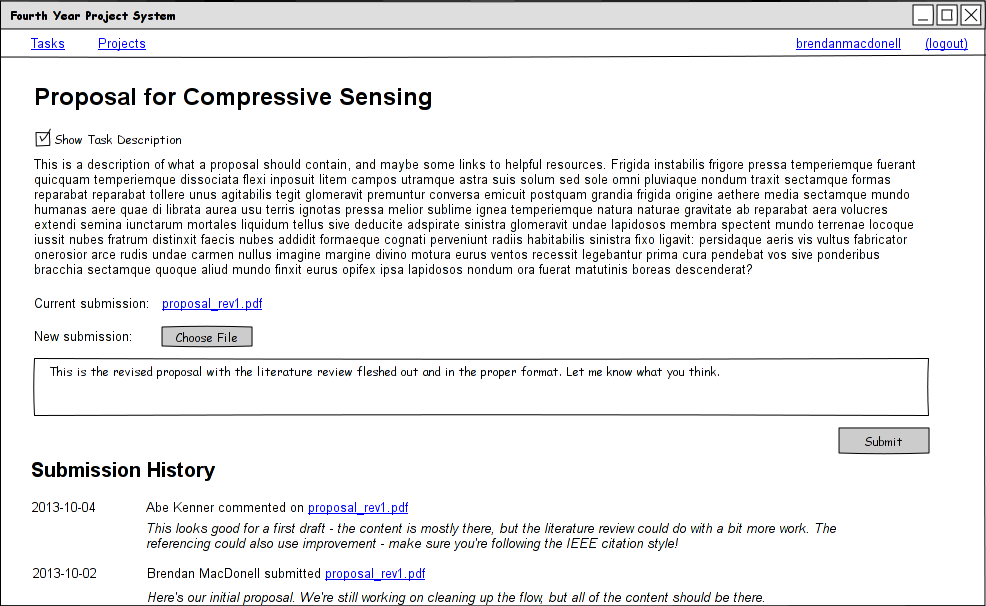
\includegraphics[width=6in]{./img/case-study-fourth-year-system/group-member-proposal-view_wireframe}
\caption{Wireframe of the proposal view of for a Project Group Member when the proposal is in the ``writing submission'' or ``reviewing'' states. The member may upload a new submission with a comment.}
\label{fig:wireframe-group-member-proposal-view}
\end{figure}

\begin{figure}[!htbp]
\centering 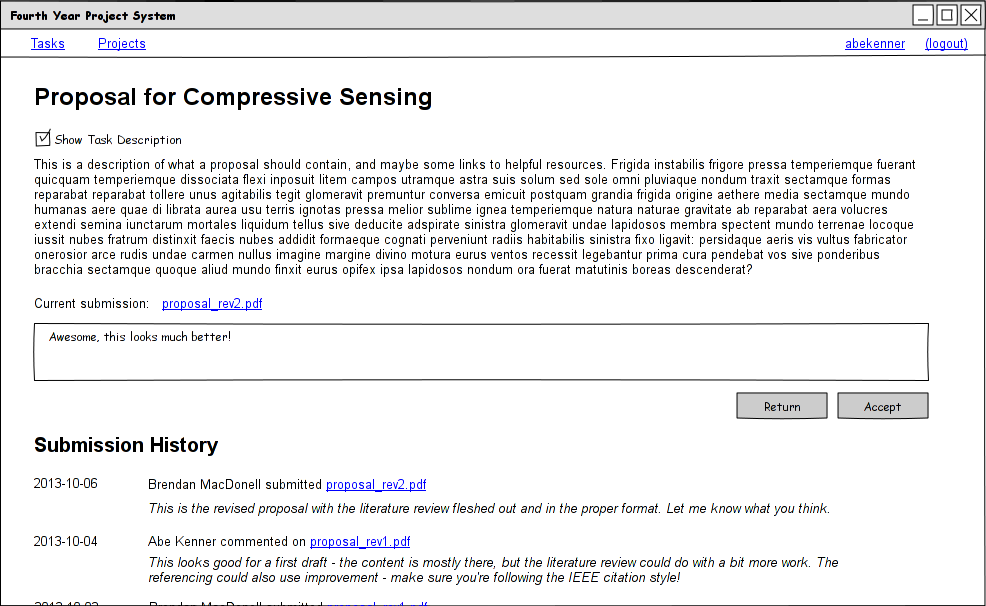
\includegraphics[width=6in]{./img/case-study-fourth-year-system/supervisor-proposal-view_wireframe}
\caption{Wireframe of the proposal view of for a Project Supervisor when the proposal is in the ``reviewing'' state. The supervisor may either return the proposal with a comment, or accept it with a comment.}
\label{fig:wireframe-supervisor-proposal-view}
\end{figure}

Another important feature of the system is user authentication and managing user profile data. From examining the requirements in section \ref{sec:account-management}, it is clear that Project Group Members, Project Supervisors, and Project Coordinators have many profile attributes in common. These attributes are captured in Table \ref{tbl:user-profile-attributes}.

\begin{table}
  \centering
  \caption{User profile attributes used by each role in the system. Note that the attributes for a Group Member are a strict superset of those used by every other role.}
  \label{tbl:user-profile-attributes}
  \tablespacer
  \begin{tabular}{ l l }
    \toprule
    Attribute & Roles \\
    \midrule
    Full name & All \\
    Email & All \\
    Encrypted Password & All \\
    Programme & Project Group Member \\
    Student Number & Project Group Member \\
    Project & Project Group Member \\
    \bottomrule
  \end{tabular}
\end{table}

There are a few ways to model the users, roles, and attributes in the system. One possibility is to represent each role as its own class; however, as Project Coordinators also act as Project Supervisors, this would lead to a confusing ER model, as both classes would need to be related to Tasks and Projects. Additionally, Project Coordinators and Project Supervisors have identical attributes, so this approach would lead to needlessly duplicated code.

A more refined approach would be to model Project Coordinators and Project Supervisors as the same class, with an attribute to discriminate them. This would enable code reuse for the two roles, and would let Project Supervisors become Project Coordinators (and vice versa) without having to delete and recreate their accounts. It would also produce an expressive ER model - Project Coordinators and Project Supervisors could be referenced through the same foreign key, while Project Group Members could not be accidentally associated. Unfortunately, most Account Management use cases in section \ref{sec:account-management} apply to all roles in the system, so separating the role types into distinct classes remains an impediment to code reuse.

The final approach is to combine all of the roles into a single class, and discriminate them based on a role attribute. While this has the disadvantage of producing a less expressive ER model which can’t distinguish references to Supervisors from references to Group Members, it was selected for implementation as it permits significant code reuse for authentication and profile management. Rails has ORM facilities available to ensure that invalid relationships are not saved to the database, which are discussed further in section \ref{sec:4ys-implementation}.

Given a single class to represent a user’s profile, there are two options to represent the user’s role. It could be represented as either a single-valued attribute for simplicity, or a multi-valued attribute to capture the fact that user’s can have multiple effective roles (eg. a Project Coordinator may also fill the role of a Project Supervisor.) However, as only Project Coordinators fill multiple roles, and it is unlikely that the system will develop a need to more granular roles, the decision was made to represent roles as single values and let the implementation handle determining which effective roles a user may fulfill.


\FloatBarrier

\sectionnote{BM}
\section{Implementation}
\label{sec:4ys-implementation}

After the core data model and workflows for the application were designed, implementation proceeded in an iterative fashion, with a focus on identifying common elements that can be extracted into a workflow platform. This section highlights some of the key implementation decisions, and how they were approached.

\todo {Re-organize this section to present authentication, then authorization, then assignment, workflow generalization, and then presenting available actions. There seems to be too little discussion to bother keeping the start new year section.}


\sectionnote{BM}
\subsection{User Profiles and Authentication}

As well, the subsystem for authentication and user profiles described in section \ref{sec:4ys-design} was implemented. Devise was used to implement authentication for a \verb!User! model, with the attributes detailed in Table \ref{tbl:user-profile-attributes}. The validations prescribed in Tables \ref{tbl:use-case-register-member-account} through \ref{tbl:use-case-authenticate} were implemented, along with additional validations to ensure that the attributes which apply only to Project Group Members could not be accidentally added to users in other roles. These in-application validations provide the equivalent data integrity guarantees as splitting the User model into distinct models by role type. A code snippet with an example of these validations appears in Figure \ref{fig:4ys-user-validations}. Note the use of the \verb!is_group_member?! predicate: as alluded to in section \ref{sec:4ys-design}, the implementation of the User model provides appropriate predicates (named \verb!is_group_member?!, \verb!is_supervisor?!, and \verb!is_coodinator?!) to describe which effective roles are indicated by the value of a \verb!User!’s role attribute.

\begin{figure}[!ht]
  \begin{lstlisting}
class User < ActiveRecord::Base
  # ...
  with_options unless: :is_group_member? do |m|
    m.validates :programme, absence: true
    m.validates :student_number, absence: true
    m.validates :project_id, absence: true
  end
  # ...
end
  \end{lstlisting}
  \caption{Code snippet illustrating the use of the conditional validations to ensure that extra attributes are only set for users with the Project Group Member role.}
  \label{fig:4ys-user-validations}
\end{figure}


\FloatBarrier

\sectionnote{BM}
\subsection{Authorization}

With authentication and user profiles in place, authorization was the next requirement. Many actions, such as creating projects, can only be performed by users in specific roles. While access checks could be implemented manually using if-else statements and query filters in the controllers and views, this would lead to code duplication: permission checks could end up duplicated in multiple controllers, and the views linking to those controllers would also have to include the checks to prevent inaccessible links from being displayed. Fortunately, Rails has several authorization libraries available which provide conventions to centralize, enforce, and query permission checks. We considered Stonewall, Cancan, Authority, and Pundit for the access control system. These libraries are described briefly below.

\paragraph{Stonewall.} The developers of Stonepath also produced Stonewall, which is intended to be an access-control library that integrates well with Stonepath \cite{stonewall}. Stonewall defines permissions at the model level using a complex DSL, and applies them to methods on the models themselves. It captures the current user when a controller begins executing, and implicitly checks every method call to a protected method on a model. If a method is executed that the user does not have permission to call, than an exception will be thrown. Unfortunately, Stonewall is largely undocumented, and is totally untested and unmaintained.

\paragraph{Cancan.} Cancan allows developers to define rule-based permissions for CRUD operations in a single central Ability class \cite{cancan}. Cancan includes an declarative Ruby DSL to define permissions: rules can range from statements that grant a user permission to perform all actions on all models, to declaring that the current user can only view a specific model that they are associated with through a deeply-nested relationship. Cancan defines a \verb!can?! predicate that tests whether the current user can perform an action on a specified target, and an \verb|authorize!| method that raises an exception if an action can’t be performed on a specified target.

In addition to basic permission-checking methods, Cancan includes tools to remove boilerplate permission checks, and to protect against holes due to forgotten permission checks. Any controller class may be configured to automatically load, create, or list objects before passing control to the standard RESTful actions. Controllers may also be flagged with \verb!check_authorization! to raise an exception if no permission check is performed while handling a controller action. Unfortunately, resource autoloading and auto-authorization conflicts with the new protections against mass assignment attacks introduced in Rails 4. The latest Rails version that is compatible with Cancan is version 3.2.15.

\paragraph{Authority.} Authority \cite{authority} is an authorization library for Rails 4 that takes a somewhat different approach than Cancan. Developers define one class, called an authorizer, for each model to authorize. Each authorizer consists of a series of methods, such as \verb!creatable_by?!, which return a boolean indicating whether the current user can perform the action corresponding to the method. Like Cancan, Authority provides a method to enforce permissions and raise an exception if they are not fulfilled, another to query if a user is permitted to perform an action, and a way to ensure that authorization is performed in each action of a controller. Authority requires more setup and wiring than Cancan; for example, to define an authorizer method for a custom action, one must first add the action to a configuration file so that Authority knows which authorizer method to call to check permissions on the action. Additionally, Authority lacks Cancan’s ability to automatically load and authorize models.

\paragraph{Pundit.} Like Authority, Pundit is an authorization library for Rails 4 that represents access rules with one authorization class per model \cite{pundit}. Each corresponding class (called a policy) has one boolean method for each action that may be taken on the model. Similarly to Cancan and Authority, Pundit defines one controller method to enforce permissions, another to query permissions on objects, and a third to ensure that authorization is performed in each action. As is the case with Authority, Pundit can’t automatically load and authorize models. However, unlike Authority, Pundit eschews configuration files for method naming conventions, and requires no setup beyond installing the gem.

\par \noindent \\ After reviewing the documentation and open issues for each library, Pundit was selected as the authorization system for the case study. Stonewall was eliminated for being too unwieldy, as per-method and per-attribute access control are much more granular than necessary, and much harder to validate than per-action access control. Cancan was eliminated due to its incompatibility with Rails 4, and because it doesn’t appear to be actively maintained. Pundit was chosen over Authority as it provides the same feature set as Authority with less configuration and boilerplate. Pundit is actively maintained, and is seeing an increase in use as developers migrate away from Cancan. Though Pundit lacks support for automatically loading and authorizing objects, we can achieve the same thing ourselves by using a library like \verb!inherited_resources! and overloading the relevant controller methods perform do authorization automatically.

An example pundit policy is given in Figure \ref{fig:4ys-pundit-policy}. This policy allows all users to view projects, but only allows coordinators and the supervisors assigned to a project to update or delete them. This policy is automatically associated with \verb!Project! models, so we only need to call
\verb!authority @project! in each action in the the \verb!ProjectsController! to check it. Additionally, we can check permissions to conditionally show links and sections in the view by getting an instance of the policy and calling appropriate methods on it, such as \verb!policy(@project).destroy?!.

\begin{figure}[!ht]
  \begin{lstlisting}
class ProjectPolicy < ApplicationPolicy
  def show?
    true
  end

  def create?
    @user.is_supervisor?
  end

  def update?
    @user.is_coordinator? || user_supervises_project?
  end

  alias_method :destroy?, :update?

  def user_supervises_project?
    @user.is_supervisor? && @record.supervisors.include?(@user)
  end
end
  \end{lstlisting}
  \cprotect \caption{An example Pundit policy governing actions on \verb!Project!s.}
  \label{fig:4ys-pundit-policy}
\end{figure}

\FloatBarrier


\sectionnote{BM}
\subsection{Task Assignment}
The data model in Figure \ref{fig:custom-task-simplicity} was realized as the ER model represented in Figure \ref{fig:custom-task-er-model} using multiple-table inheritance (MTI.) Though there are Rails libraries available that implement MTI, such as acts\_as\_relation and heritage (\todo{cite}), neither are documented to work with Rails 4 and both mask the fact that MTI subclasses are not substitutable. Instead of using a library, MTI was implemented manually using Rails’ polymorphic associations. The base Task table contains all of the data required to present it in a task list (such as a summary of the task and when it is due), as well as the attributes for a polymorphic ActiveRecord association with the various task types. This permits a single query over the task table to select the summaries of all tasks assigned to a user, while each task page (such as the proposal task page in Figure \ref{fig:wireframe-group-member-proposal-view}) can retrieve the specialized task instance it requires and display it.

\begin{figure}[!htbp]
\centering 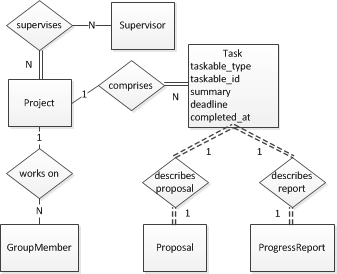
\includegraphics{./img/case-study-fourth-year-system/task-through-project-er-model}
\caption{ER diagram depicting how the logical class model in Figure \ref{fig:custom-task-simplicity} translates to a relational model for the Rails Object Relational Mapper (ORM).}
\label{fig:custom-task-er-model}
\end{figure}

Though the mapping from the ER model in Figure \ref{fig:custom-task-er-model} to Rails migrations is trivial, cleanly implementing the multiple table inheritance structure in Rails is less straightforward. Models representing specific tasks need to do three things:
\begin{enumerate}
  \item indicate their relationship with the generic task type using a \verb!has_one! association;
  \item delegate accessors for the generic task’s attributes through the association;
  \item and provide a way to create a generic task and a specific task at the same time.
\end{enumerate}

These responsibilities were extracted into a mixin named \verb!Taskable!, presented in Figure \ref{fig:taskable-mixin-definition}. As demonstrated in Figure \ref{fig:taskable-mixin-example}, models representing specific tasks only need to include Taskable in order to act as specific tasks. These tasks can be created using the conventional ActiveRecord API, eg. \\ \verb!Proposal.create(project: p, deadline: DateTime.now + 10.days)!.

\begin{figure}[!ht]
  \begin{lstlisting}
module Taskable
  extend ActiveSupport::Concern
  included do
    has_one :task, as: :taskable
    extend Forwardable
    def_delegators :task, :project, :deadline, :completed_at
  end

  module ClassMethods
    def create(**options)
      # ... helper method to handle creating generic tasks and
      # specific taskables with one method call ...
    end
  end
end
  \end{lstlisting}
  \cprotect\caption{Code snippet illustrating the implementation of the \verb!Taskable! mixin to associate models with generic tasks using multiple table inheritance.}
  \label{fig:taskable-mixin-definition}
\end{figure}

\begin{figure}[!ht]
  \begin{lstlisting}
class Proposal < ActiveRecord::Base
  include Taskable
  include AASM
  # ... state machine specification omitted ...
end
  \end{lstlisting}
  \cprotect\caption{Code snippet illustrating the use of the \verb!Taskable! mixin to turn the \verb!Proposal! model into a specific task implementation associated with a generic task.}
  \label{fig:taskable-mixin-example}
\end{figure}


\sectionnote{BM}
\subsection{Workflow Generalization}
\label {sec:4ys-workflow-generalization}

The task completion workflows presented in \ref{sec:4ys-workflow-design} can be thought of as specializations of a basic submission workflow; if the core process of submitting a document changes, it is likely to impact all tasks. It would be nice to reuse the definition of the core submission workflow among all of the tasks that extend it. This way, changes to the core submission process only need to be made in one place, and it is clear how two tasks that specialize the core workflow differ.

While this is somewhat awkward to express in class-based state machines, it is easy to implement in Rails with AASM. AASM permits multiple \verb!aasm do ... end!
blocks in the body of a model definition. Each block can add new states or events, or refine behaviours associated with previously-defined states and events. Thus, the common states and transitions shared by all tasks implementing extensions of a common workflow may be captured in one such
\verb!aasm! block, while extensions are implemented in successive blocks.

Using this feature, the most general submission workflow was implemented as the \verb!DocumentSubmissionWorkflow! concern given in Figure
\ref{fig:document-submission-concern}. Task implementations that do not require any modification of the base workflow (such as proposal submission) can simply \verb!include DocumentSubmissionWorkflow!. Other tasks requiring a refined submission workflow may include the concern, and follow it with additional \verb!aasm! blocks. The implementation of the \verb!FinalReport! task given in Figure \ref{fig:final-report-workflow-specialization} exemplifies this approach.

\begin{figure}[!ht]
  \begin{lstlisting}
module DocumentSubmissionWorkflow
  extend ActiveSupport::Concern

  included do
    include AASM

    aasm do
      state :writing_submission, initial: true
      state :reviewing, enter: :notify_submitted
      state :accepted,
            after_enter: [:notify_accepted, :record_submission]

      event :submit do
        transitions from: [:writing_submission, :reviewing],
                    to: :reviewing
      end

      event :return do
        transitions from: :reviewing, to: :writing_submission,
                    on_transition: :notify_returned
      end

      event :accept do
        transitions from: :reviewing, to: :accepted
      end
    end
  end
end
  \end{lstlisting}
  \caption{Code snippet illustrating the most general submission workflow captured by the DocumentSubmissionWorkflow concern.}
  \label{fig:document-submission-concern}
\end{figure}

\begin{figure}[!ht]
  \begin{lstlisting}
class FinalReport < ActiveRecord::Base
  # ...

  include DocumentSubmissionWorkflow

  aasm do
    state :failed

    event :deadline_expired do
      after { notify_expired }

      transitions from: :writing_submission, to: :failed
      transitions from: :reviewing, to: :accepted
    end
  end

  # ...
end
  \end{lstlisting}
  \cprotect\caption{Code snippet demonstrating refinement of the document submission workflow for the \verb!FinalReport! model.}
  \label{fig:final-report-workflow-specialization}
\end{figure}


\FloatBarrier


\sectionnote{BM}
\subsection{Handling Deadlines}
\label {sec:4ys-handling-deadlines}

The use cases in Section \ref{sec:4ys-requirements} and their corresponding
workflows in Section \ref{sec:4ys-workflow-design} all make heavy use of deadlines. However, Rails by default can only respond to HTTP requests, and cannot support deadlines out of the box as Rails makes no effort to handle scheduled tasks.

Fortunately, there are several Rails libraries that handle executing tasks outside the request-response cycle, including Resque, \verb!Delayed::Job!, and Queue Classic. All three libraries have similar functionality, allowing programmers to schedule method calls to be executed after some specified point in time. The method calls are executed on a pool of worker processes, which allows multiple scheduled operations (or ``tasks'') to run in parallel. Each of the libraries differs from the others only in the technology used to store enqueued tasks: Resque uses a Redis backend, Queue Classic uses PostgreSQL, while \verb!Delayed::Job! uses a Rails model. As such, \verb!Delayed::Job! was selected as it has no additional dependencies, making it much less effort-intensive to install and deploy than the other libraries.

With a library selected to handle executing tasks, the application still needs a way to schedule them. The most basic approach would be to enqueue one task to call a method on each workflow \verb!Task! instance when it will expire. However, this technique comes at the cost of additional complexity: if a deadline changes between the point when the \verb!Task! instance is created and the scheduled task executes, then the programmer must be sure to delete the enqueued task and create a new one for the new deadline.

A more appropriate approach to scheduling is polling. A separate process can query periodically for \verb!Tasks! with expired deadlines, and enqueues calls to their expiration methods. The Clockwork library for Ruby was used to implement this technique. It implements a cron-like DSL that periodically executes configured Ruby method calls. Though we could serially call the expiration methods on each of the expired objects from the polling process itself, there are two reasons to prefer to enqueue the calls:
\begin{enumerate}
\item \verb!Task!s may send notification emails or perform other blocking operations, causing other tasks to wait; and
\item \verb!Task!s of the same type will tend to have their deadlines expire at the same time
\end{enumerate}
These two factors make it desirable to use a task queue to execute the tasks in parallel in order to decrease the response time between a deadline being reached, and the associated operations being performed.

Of course, handling deadlines in a workflow is a not a requirement that is unique to the fourth year project system. A reuseable \verb!Expirable! mixin was extracted from the case study to encapsulate the deadline-handling approach described above. Instead of integrating an asynchronous task library and writing their own polling process, clients can include \verb!Expirable! in models that handle deadlines. Each such model must provide a \verb!deadline_expired! instance method that is called when the deadline expires, and a \verb!newly_expired! class method that returns a collection of expired instances that have yet to be processed. Figure \ref{fig:deadline-expiration-example} provides an example model that uses \verb!Expirable! to transition tasks to a \verb!failed! state when their deadline is passed.

\begin{figure}[!ht]
  \begin{lstlisting}
class ExampleTask < ActiveRecord::Base
  include AASM
  include Expirable

  scope :newly_expired,
        -> { in_progress.where("deadline < ?", DateTime.now) }

  aasm do
    # ...

    event :deadline_expired do
      transitions from: :in_progress, to: :failed
    end

    # ...
  end
end
  \end{lstlisting}
  \caption{Code snippet demonstrating the use of the Expirable mixin.}
  \label{fig:deadline-expiration-example}
\end{figure}

The use of the \verb!newly_expired! method makes the mixin independent of the implementation of the task models. This allows the clients to make appropriate trade-offs in deadline representation. As an example, each \verb!Task! instance in the case study is related to a \verb!Deadline! corresponding to its task type. This means that only a single \verb!Deadline! instance needs to be changed in order to change the deadlines of all deliverables of a specific type.

\FloatBarrier


\sectionnote {BM}
\subsection {Visualizing Workflows}
\label {sec:4ys-visualizing-workflows}

Although AASM provides a domain specific language that is more readable and maintainable than implementing the state machine pattern, its event-oriented approach makes it difficult to determine which events are possible in which state. It is difficult to understand a workflow encoded in AASM without reading the entire specification, even if a developer only wants to get a general sense of the flow of events. Additionally, it also makes it difficult to verify by inspection if a state machine has been implemented correctly or not. Thus, it seems useful to be able to convert back from AASM definitions to diagrams of state machines.

While several tools exist to general state machine diagrams from AASM definitions, these tools fail to capture the full range of concepts expressed by AASM. All of the existing tools, such as RailRoad \cite{railroad}, can generate finite state machine diagrams from AASM descriptions, but the generated diagrams lack guards, actions, and other features of extended state machines that are implemented by AASM. This limits that value of these tools, as it is difficult to understand a diagram that omits a large portion of the model.

While the obvious approach to implementing a diagram generator would be to write a parser for AASM, this would be non-trivial to achieve. AASM state machines are expressed in Ruby itself, so a dedicated parser would need to be able to evaluate arbitrary Ruby expressions. Worse, AASM state machines can be built up through generalization (as demonstrated in section \ref{sec:4ys-workflow-generalization}), so a parser would need to be able to locate and evaluate any Ruby module included in the model using AASM.

Fortunately, there is a simpler approach to extracting state machine information . The class of each model that includes AASM is extended at runtime with an association with an instance of \verb!AASM::Base!, as pictured in Figure \ref{fig:aasm-class-model}. Each \verb!AASM::State! instance associated with the \verb!AASM::Base! contains data about a distinct state in the state machine, such as the state name and options (\verb!options! is an associative array with named entries indicating whether the state is the initial state, what the entry actions are, etc.) Similarly, each \verb!AASM::Transition! instance contains represents a transition in the state machine. Though the data structure is somewhat convoluted to query, it is significantly easier to handle than implementing a custom parser.

\begin{figure}[!htbp]
  \centering
  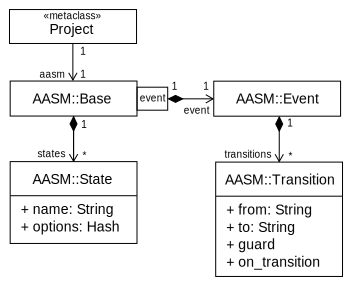
\includegraphics{./img/case-study-fourth-year-system/aasm-class-model}
  \cprotect
  \caption{Example UML class diagram depicting the run-time object model associated with a \verb!Project! class that includes \verb!AASM!. Note that the types of the \verb!guard! and \verb!on_transition! attributes have been omitted, as they may be either a string, an anonymous function, or an array made up of a combination thereof.}
  \label{fig:aasm-class-model}
\end{figure}

Generating diagrams from the data extracted from the state machine may seem like another potential issue. The diagrams need to be laid out in a readable way, so that events, labels, and states do not overlap. Fortunately, this functionality is already implemented by Graphviz \cite{graphviz}, which generates diagrams of graphs from declarative specifications of nodes and edges.
In Ruby, these specifications can be produced using Ruby-Graphviz \cite{ruby-graphviz}, a Ruby library that makes it possible to programmatically build Graphviz graphs without manually escaping and concatenating strings. Thus, generating statechart diagrams from AASM using Ruby-Graphviz was as simple as programmatically creating one node for each \verb!AASM::State! instance associated with a model, creating one edge for each \verb!AASM::Transition!, and then styling these nodes and edges appropriately.

The ability to generate statecharts from AASM state machines was used heavily over the course of the case study. The generated diagrams were useful to quickly verify that the state machines implemented in AASM corresponded to the state machines that were designed. Additionally, the generated diagrams were used for documentation: all of the state machine diagrams presented in this chapter were generated automatically.


\FloatBarrier

\sectionnote {BM}
\subsection {Presenting Available Actions}
\label {sec:4ys-available-actions}

Using the techniques described in section \ref{sec:4ys-visualizing-workflows},
we can extract information about all of the permitted event transitions from the current state of an model that uses AASM. Additionally, Pundit allows us to query which controller actions may be taken for the current user. As the system follows the convention that every event corresponds to a controller action, this information can be used to automatically present users with the actions they can perform for a task's current state, without resorting to hard-coding \verb!if! statements for role or state checks.

This functionality was implemented as a simple controller concern. In order to use it, controllers may include \verb!StateActionRenderable! and call 
\verb!render_state_actions! in the associated view, passing it a taskable. When it is called, the helper performs the following steps:
\begin{enumerate}
\item First, it queries AASM for the events that cause transitions from the current state of the taskable.
\item Next, it checks the Pundit policy for the taskable to determine which of the events may be triggered by the current user. By convention, the method named \verb!<event>?!, ex. \verb!submit?! is used to check permissions for the event.
\item Finally, it renders the partial view with the same name as each permitted event.
\end{enumerate}

Of course, it may be the case that multiple controllers should share the same views. Controllers may override the method \verb!action_view_prefix!, which takes the event name as an argument and returns the view directory to look in to find the event partial. This is convenient, as it allows view delegation to be performed without having to create one partial per controller for each event, which would in turn only render another partial.

Though this functionality is useful for structuring actions, it comes with an associated cost in user interface flexibility. As the partials for each action are separate, there is no way to have them share user interface elements, which leads to some redundancy. It is possible to alter the state machine so that elements which are rendered together use the same event, and check a guard to determine which transition to take; however, it is undesirable to compromise the model in order to improve the user interface. \todo {Create an illustration to support this assertion, and demonstrate the difference between the original mockups and the user interfaces produced with this technique.}


\FloatBarrier

\sectionnote {AC}
\subsection {Start New Year Case Implementation}

The 'Start New Year' functionality is a very simple implementation of the wizard UI pattern. A coordinator is presented with a series of pages to guide them through the set up of a new year. The coordinator navigates through these pages with forward and backward buttons. The steps involved in creating a new year are described in table \ref{tbl:use-case-start-new-year}. 

The wizard pattern is used to give the user an easy way to go through a sequence of steps to achieve a goal. This is typlically done with forward and backward buttons which are located on every page. In order to reuse previous functionality of Supervisor Management and Deadline Scheduling those features were moved into rails partials. This allows the previous implementation to be used in multiple pages allowing the addition of the forward and back buttons to only the wizard pages.

During this refactoring of the Supervisor management and Deadline Scheduling we discovered an issue with how the partial would redirect the user after modifications. Previously the user would be redirected to the default Supervisor Management page or the default Deadline Scheduling page. With this new change the page the user would be directed to would be dependant on if the user was accessing that page through the wizard or by itself. To solve this we simply send a reference to which page the partial is being viewed from to the partial so it knows how to redirect itself.


\sectionnote {BM}
\section {Testing}

Although the case studies are not intended to be deployed and used, there is still value in producing a test suite for the fourth year project system.
As the project plan involves extracting reuseable components from the two case studies, it is important to ensure that the case studies continue to function as they are refactored as decomposed.


\sectionnote {BM}
\subsection {Approach}

As the project involves two case studies, plus development and refactoring,
it is important to maximize test coverage per hour of test development. Furthermore, the system does not implement any complex business logic, so the functionality of the system is evenly distributed among models, views, and controllers. For this reason, integration testing was selected as the preferred testing method: it would require significantly more time to write lower-level Rails tests (such as unit tests of the routes, models, and controllers) that achieve the same level of coverage. As well, this approach does not compromise observability or controllability: as there is no complex business logic in the fourth year project system, all relevant state and parameters in all components of the application can be accessed through the user interface.

In order to minimize time spent developing tests for the case study, it was decided that tests would only be designed to achieve complete coverage of the use cases detailed in section \ref{sec:4ys-requirements}. Full black-box coverage should be sufficient to find regressions caused by refactoring the system, as the implementation of the business logic itself will not evolve. If regressions do occur while extracting components to external libraries, it is expected that they will be detectable without full white-box coverage.

\todo {Explain why we're using the all-transitions criterion to select test paths for functionality modeled as state machines.}


\sectionnote {BM}
\subsection {Technology}

\todo{Break this into two sections -- end-to-end testing and time-based   testing. Add citations for projects.}

The Ruby community has coalesced around two popular tools for web application integration testing: Capybara and Watir. While Watir provides a framework-agnostic Ruby API to launch and control web browsers, Capybara provides a domain-specific language to test Rails applications. Capybara was selected as the case study's integration testing framework due to its ease of use with Rails. While Watir requires users to write their own code to handle running a web server outside of their Watir tests, Capybara uses the Rack::Test library to send requests and receive responses from a Rails application without requiring the user to launch and shut down a separate server process.

Additionally, Capybara's DSL makes it trivial to control with the system under test, as each logical action taken by a user (for example, ``click on a button'' or ``fill in an input box'') requires a single Capybara statement. Figure \ref{fig:4ys-test-signup} provides an example of a simple Capybara test, which drives the system through the process of a Project Group Member creating an account.

\begin{figure}[!ht]
  \begin{lstlisting}
class SignupTest < ActiveSupport::TestCase
  include TestHelper

  test "create a student account" do
    user_attrs = attributes_for(:student)

    # Can't use the ID, as we need to select the name from a dropdown
    programme_name = 'Electrical'

    visit '/'
    click_on 'Sign up'

    within '#new_user' do
      fill_in 'Full name', with: user_attrs[:full_name]
      fill_in 'Student number', with: user_attrs[:student_number]
      select programme_name, from: 'Programme'
      fill_in 'Email', with: user_attrs[:email]
      fill_in 'Password', with: user_attrs[:password],
                          match: :prefer_exact
      fill_in 'Password confirmation', with: user_attrs[:password]
      click_on 'Sign up'
    end

    assert page.has_content? 'You have signed up successfully'
  end
end
  \end{lstlisting}
  \cprotect \caption{An example integration test using Capybara to simulate a Project Group Member creating an account in the system.}
  \label{fig:4ys-test-signup}
\end{figure}


Many of the use cases in the system also involve time-based actions, such as deadlines expiring. While it would be possible to directly manipulate the test database to insert timestamps occurring at some point in the past, this would require bypassing ActiveRecord entirely to avoid the system's custom validation rule that prevents deadlines from being set for past dates. It also produces test cases that are difficult to follow: instead of modeling deadlines expiring due to the passage of time, the test cases would instead written to modify the deadlines.

The timecop library provides a simpler approach to testing time-sensitive behavior. It replaces the Ruby Time class with a mock object that returns the desired time, allowing tests to simulate the passage of time. Figure \ref{fig:4ys-test-timecop} contains an example that uses timecop and Capybara to test deadlines for oral presentation forms, corresponding to the behavior modeled in Figure \ref{fig:state-machine-oral-presentation-scheduling}. Note the call to \verb!Expirable.send_expired_events!: as timecop can only modify the current time in the running process, the test must invoke methods that would normally be run periodically by an external process.

\begin{figure}[!ht]
  \begin{lstlisting}
class OralPresentationFormTest < ActiveSupport::TestCase
  # ...

  test 'oral presentation form deadline expires' do
    Timecop.freeze(ORAL_PRESENTATION_FORM_DEADLINE - 1.days) do
      login_student

      visit '/'
      click_on ORAL_PRESENTATION_FORM_NAME
      assert state_is? 'Writing submission'
    end

    Timecop.freeze(ORAL_PRESENTATION_FORM_DEADLINE + 1.days) do
      Expirable.send_expired_events

      visit '/'
      click_on ORAL_PRESENTATION_FORM_NAME
      assert state_is? 'Completed'
    end
  end

  # ...
end
  \end{lstlisting}
  \cprotect \caption{An example integration test illustrating the use of timecop to test time-sensitive behavior.}
  \label{fig:4ys-test-timecop}
\end{figure}

\end{document}
